% This file should contain text on the baseline design process and tools used by RVLT/Chris Silva for comparison to our new MDAO design process
% This section is assigned to Justin

Add a description of the traditional process and tools used by Chris Silva and team for developing the 3 UAM vehicle designs.  Include an XDSM of the traditional process.  

General outline for this section:
\begin{itemize}
    \item Traditional process used by RVLT for initial concept development applied different disciplinary tools in a linear/sequential fashion
    \item NPSS used to create cycle model and engine surrogate model
    \item CAMRAD used to model the rotors
    \item ...tools for other disciplines...
    \item NDARC used to determine mission performance
    \item Optimization/iterations completed using this tool set to generate initial designs
    \item Challenges:
    \begin{itemize}
        \item Process does not include detailed models for some disciplines (electrical?)
        \item Existing tool set does not provide capabilities for completing large scale gradient-based optimization to further refine the designs
    \end{itemize}
\end{itemize}


\begin{figure}[htb]
\begin{center}
 % \textbf{!!!!! Create XDSM of Traditional Process !!!!!}
 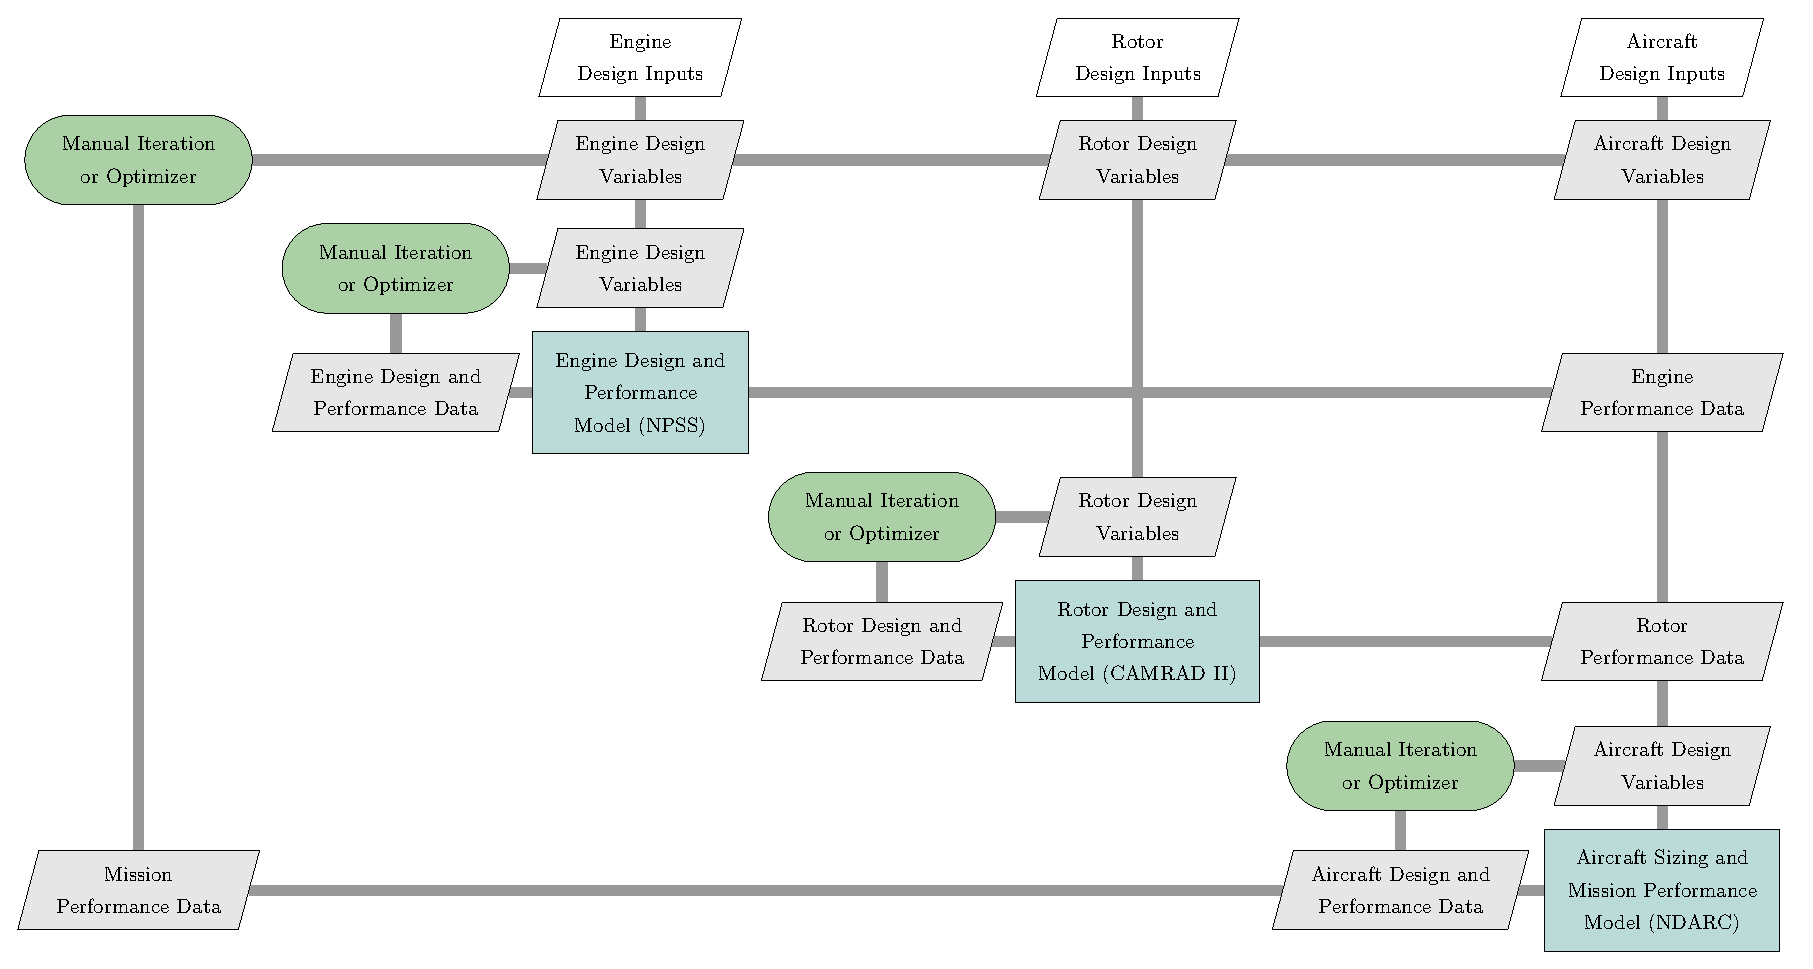
\includegraphics[width=1.0\textwidth]{../Images/Traditional_XDSM.pdf}
 \caption{Traditional Conceptual Design Process.}
 \label{f:trad_XDSM}
\end{center}
\end{figure}

